\section{Рисунки и алгоритмы их генерации}\label{sec:figures}

Восемь рисунков ниже --- не украшение: каждый изображает реальный объект
изложения (центры $6m\pm1$, их простые ранги, old-peel-генеалогию спуска) и
воспроизводим из публичного исходника. Мы собираем их здесь, в
приложенческом стиле, и для каждого приводим порождающую функцию и точную
конструкцию. Рисунки~\ref{fig:old-peel-tree}--\ref{fig:genealogy-ornament} взяты
из \srcpath{tools/fractal/euclid\_fractal.py}; два космологических вида,
рисунки~\ref{fig:observer-horizon}--\ref{fig:time-sphere}, --- из
\srcpath{tools/fractal/euclid\_cosmology.py}. Оба рисуют один и тот же
математический объект (шаг $6k\mp1=p\,(6t\pm1)$); второй файл лишь размещает
его для космологического прочтения. Все цвета, палитры и пиксельная геометрия,
названные ниже, --- параметры matplotlib, а не математические утверждения.

\begin{figure}[htbp]
  \centering
  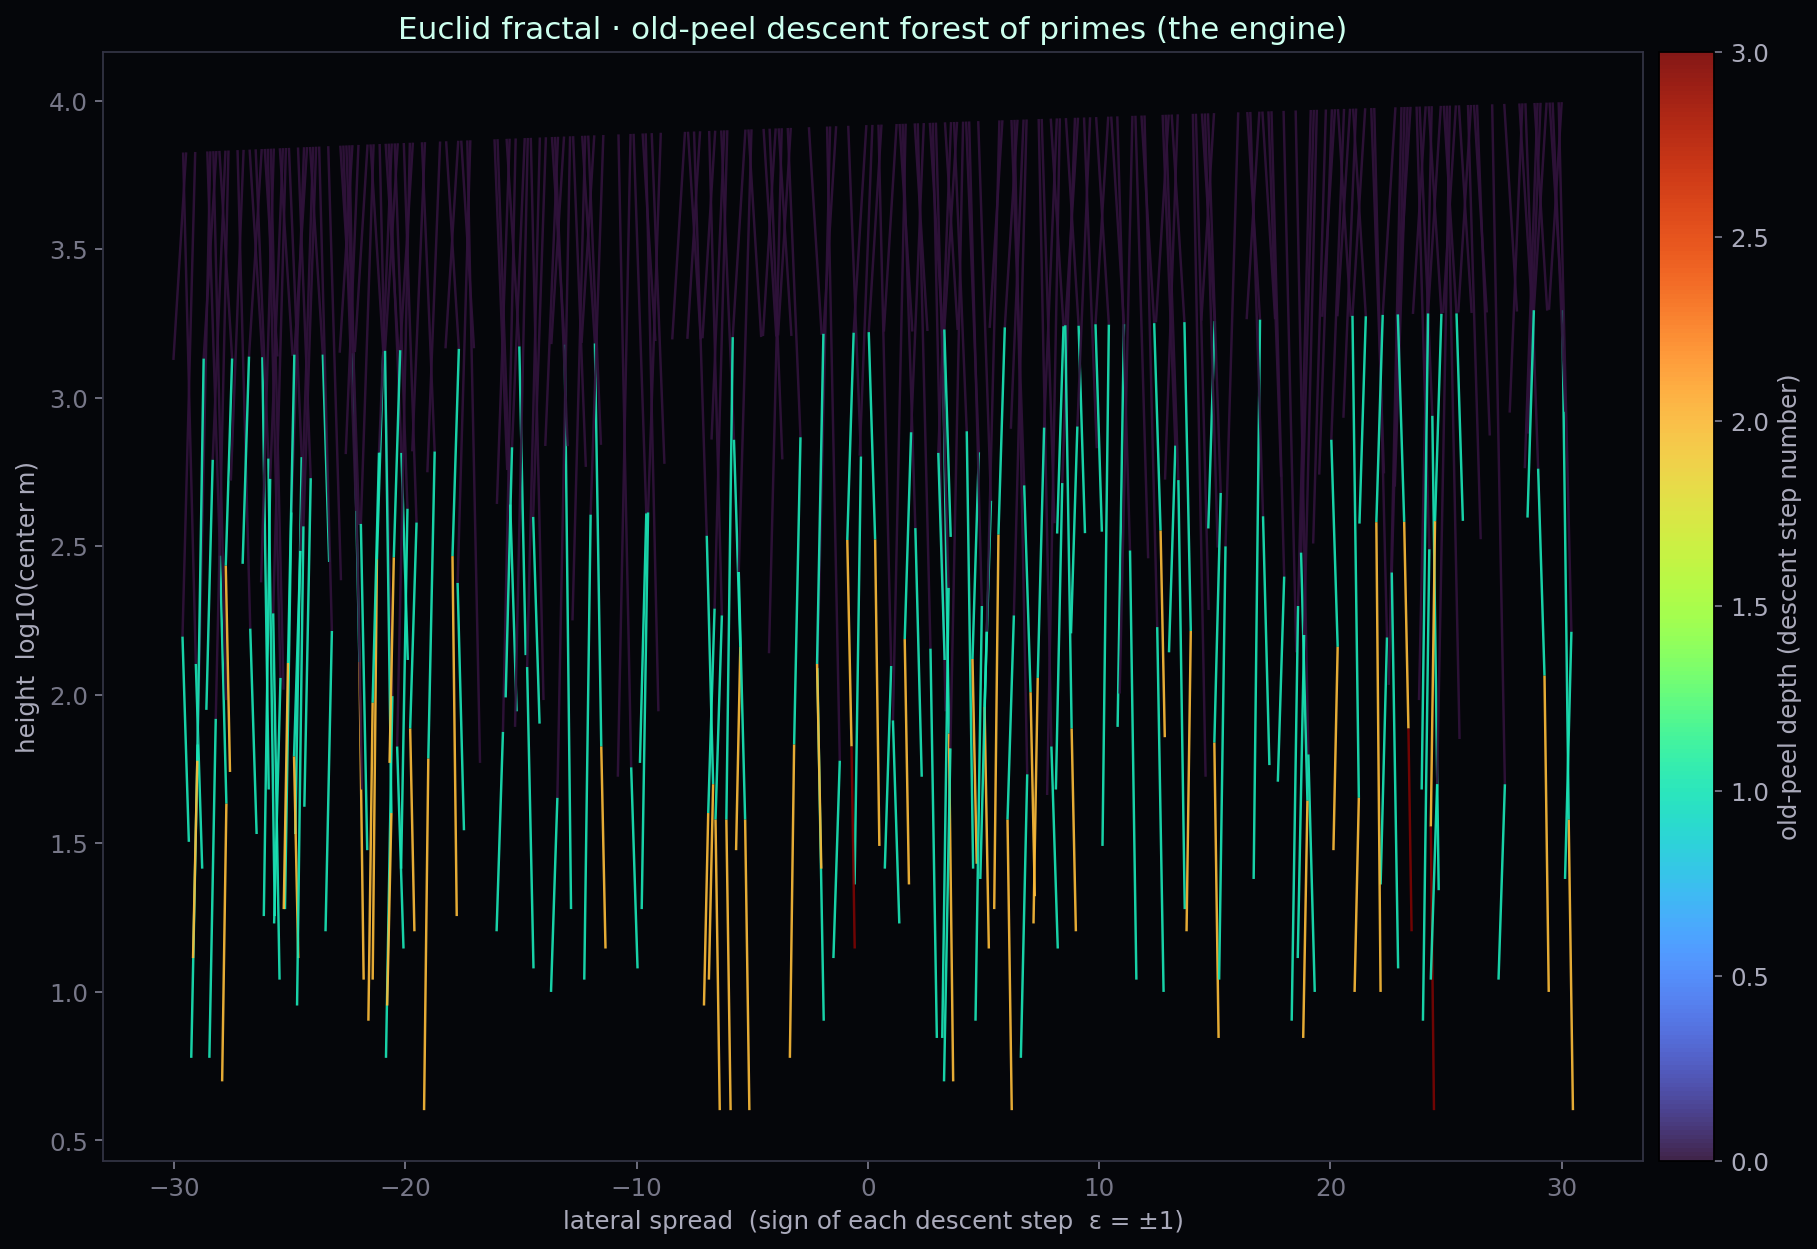
\includegraphics[width=\linewidth]{figures/1_old_peel_tree.png}
  \caption{Old-peel-лес спуска простых --- сам двигатель, запущенный рекурсивно
  из ряда крупных центров.}
  \label{fig:old-peel-tree}
\end{figure}

\emph{Алгоритм генерации (рис.~\ref{fig:old-peel-tree}).} Источник:
\srcpath{tools/fractal/euclid\_fractal.py::old\_peel\_tree}. Фиксируем $A=200$ и
просеиваем все простые до $4A^2$; пул пойманных простых --- простые $p$ с
$3<p\le A$. Разместим горизонтальный ряд из $460$ корней с абсциссами $x$,
равномерно распределёнными по $[-30,30]$; $i$-й корень несёт центр
$n=\lfloor A^2/6\rfloor+7i$. Из каждого корня запускается рекурсивный спуск
$\mathrm{peel}(n,\varepsilon,d,x)$ для обоих знаков $\varepsilon=\pm1$: он
останавливается при глубине $d>7$ или $n<2$; требует, чтобы сторона
$a=6n+\varepsilon$ была простым с $a>A$; берёт противоположную сторону
$6n-\varepsilon$, находит первое простое $p$ из пула, делящее её, образует
частное $q=(6n-\varepsilon)/p$, читает его знак $\delta$ по $q\bmod6$
($\delta=+1$ при $q\equiv1$, $\delta=-1$ при $q\equiv5$, иначе обрыв) и задаёт
дочерний центр $t=(q-\delta)/6$ (обрыв при $t\le0$). Шаг рисует отрезок из
$(x,\ \log_{10}(n+1))$ в $(x+\varepsilon\cdot0.55/(d+1),\ \log_{10}(t+1))$, затем
рекурсивно заходит в $t$ с обоими знаками на глубине $d+1$. Вертикальная ось ---
высота $\log_{10}(\text{центр})$; горизонтальный сдвиг кодирует знак спуска
$\varepsilon$; отрезки окрашены по глубине спуска $d$ (палитра turbo).

\begin{figure}[htbp]
  \centering
  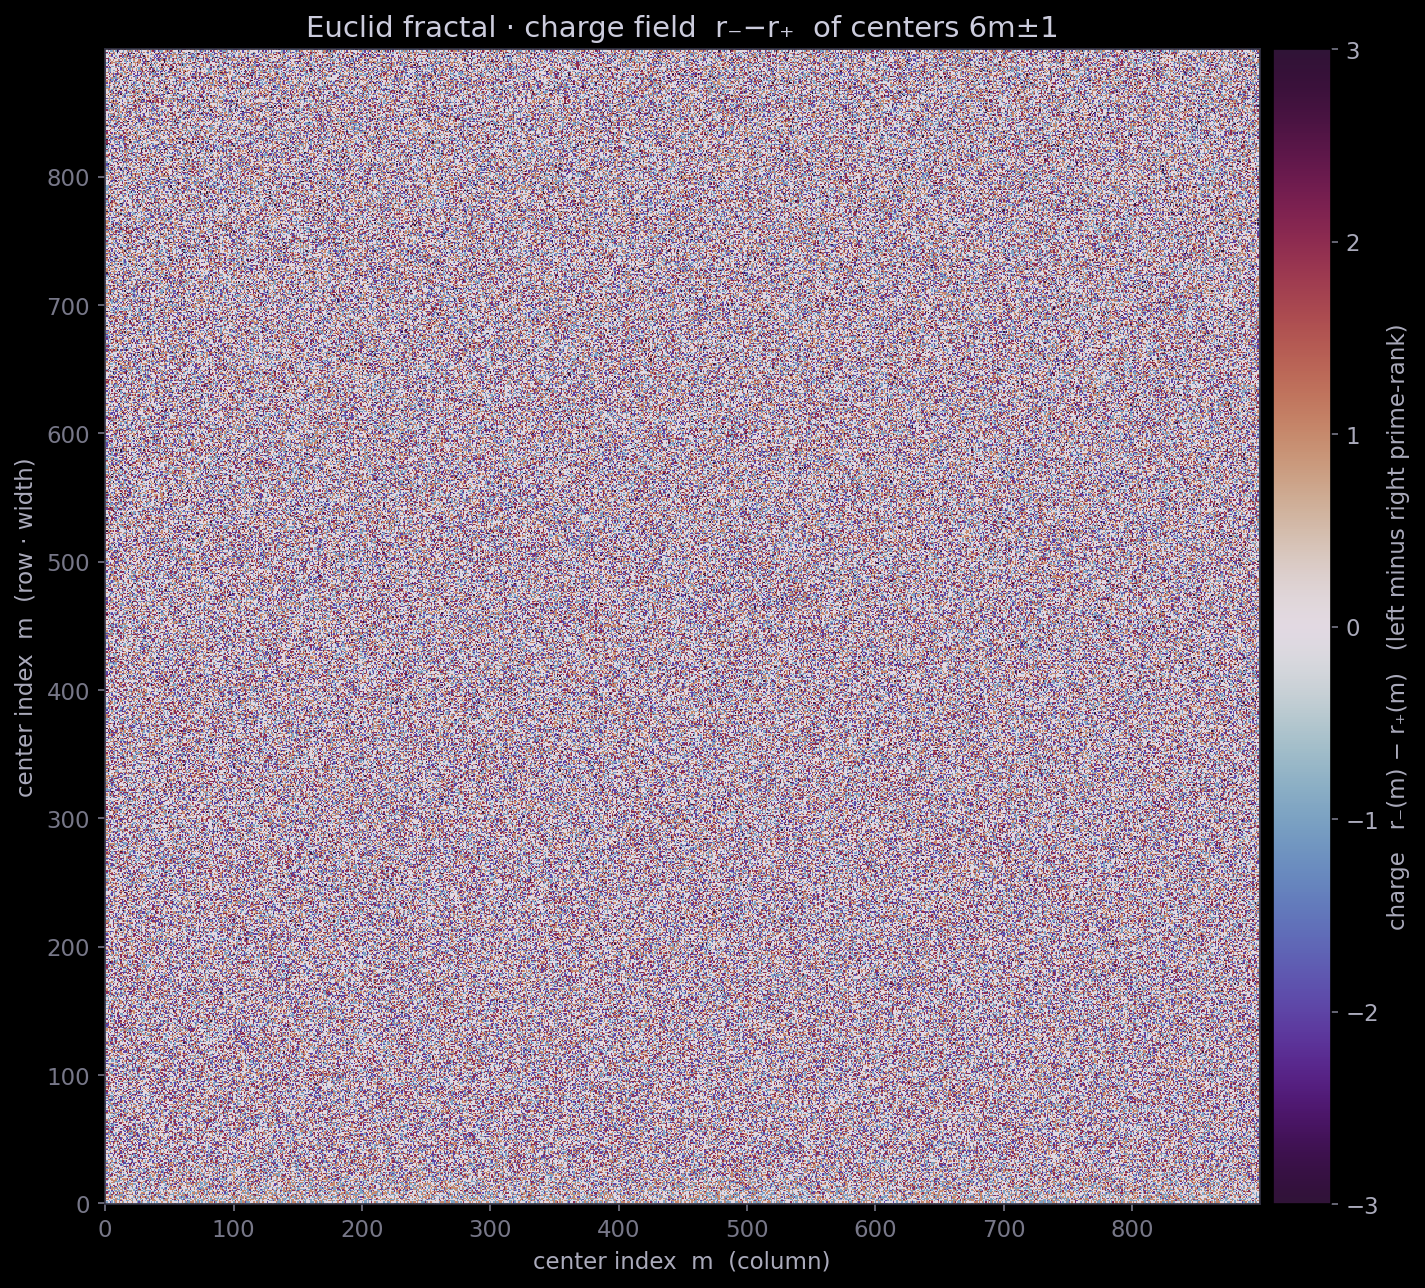
\includegraphics[width=\linewidth]{figures/2_rank_field.png}
  \caption{Поле заряда $r_-(m)-r_+(m)$ центров $6m\pm1$: фрактальная порождающая
  функция простого ранга.}
  \label{fig:rank-field}
\end{figure}

\emph{Алгоритм генерации (рис.~\ref{fig:rank-field}).} Источник:
\srcpath{tools/fractal/euclid\_fractal.py::rank\_field}. Параметры $A=60$, $W=900$;
слой простых --- $\{p:\ A<p\le A^2\}$. Для каждого центрального индекса
$m\in\{0,\dots,W^2-1\}$ считаются два ранга: $r_-(m)$ --- число простых слоя,
делящих нижнюю сторону $6m-1$, и $r_+(m)$ --- верхнюю сторону $6m+1$. Для каждого
$p$ решается сравнение $6m\equiv\pm1\pmod p$ через обратный элемент
$6^{-1}\bmod p$, дающий корень $r\equiv\pm6^{-1}\pmod p$, стартовое смещение
$(r-1)\bmod p$ и единицу, прибавляемую к каждой $p$-й позиции массива $r_\mp$.
Изображается заряд $r_-(m)-r_+(m)$: вектор длины $W^2$ переформатируется в
матрицу $W\times W$ (строка $=\lfloor m/W\rfloor$, столбец $=m\bmod W$) и
рисуется расходящейся палитрой twilight-shifted (противоположные знаки заряда на
двух концах, ноль --- центр), с нижним началом координат.

\begin{figure}[htbp]
  \centering
  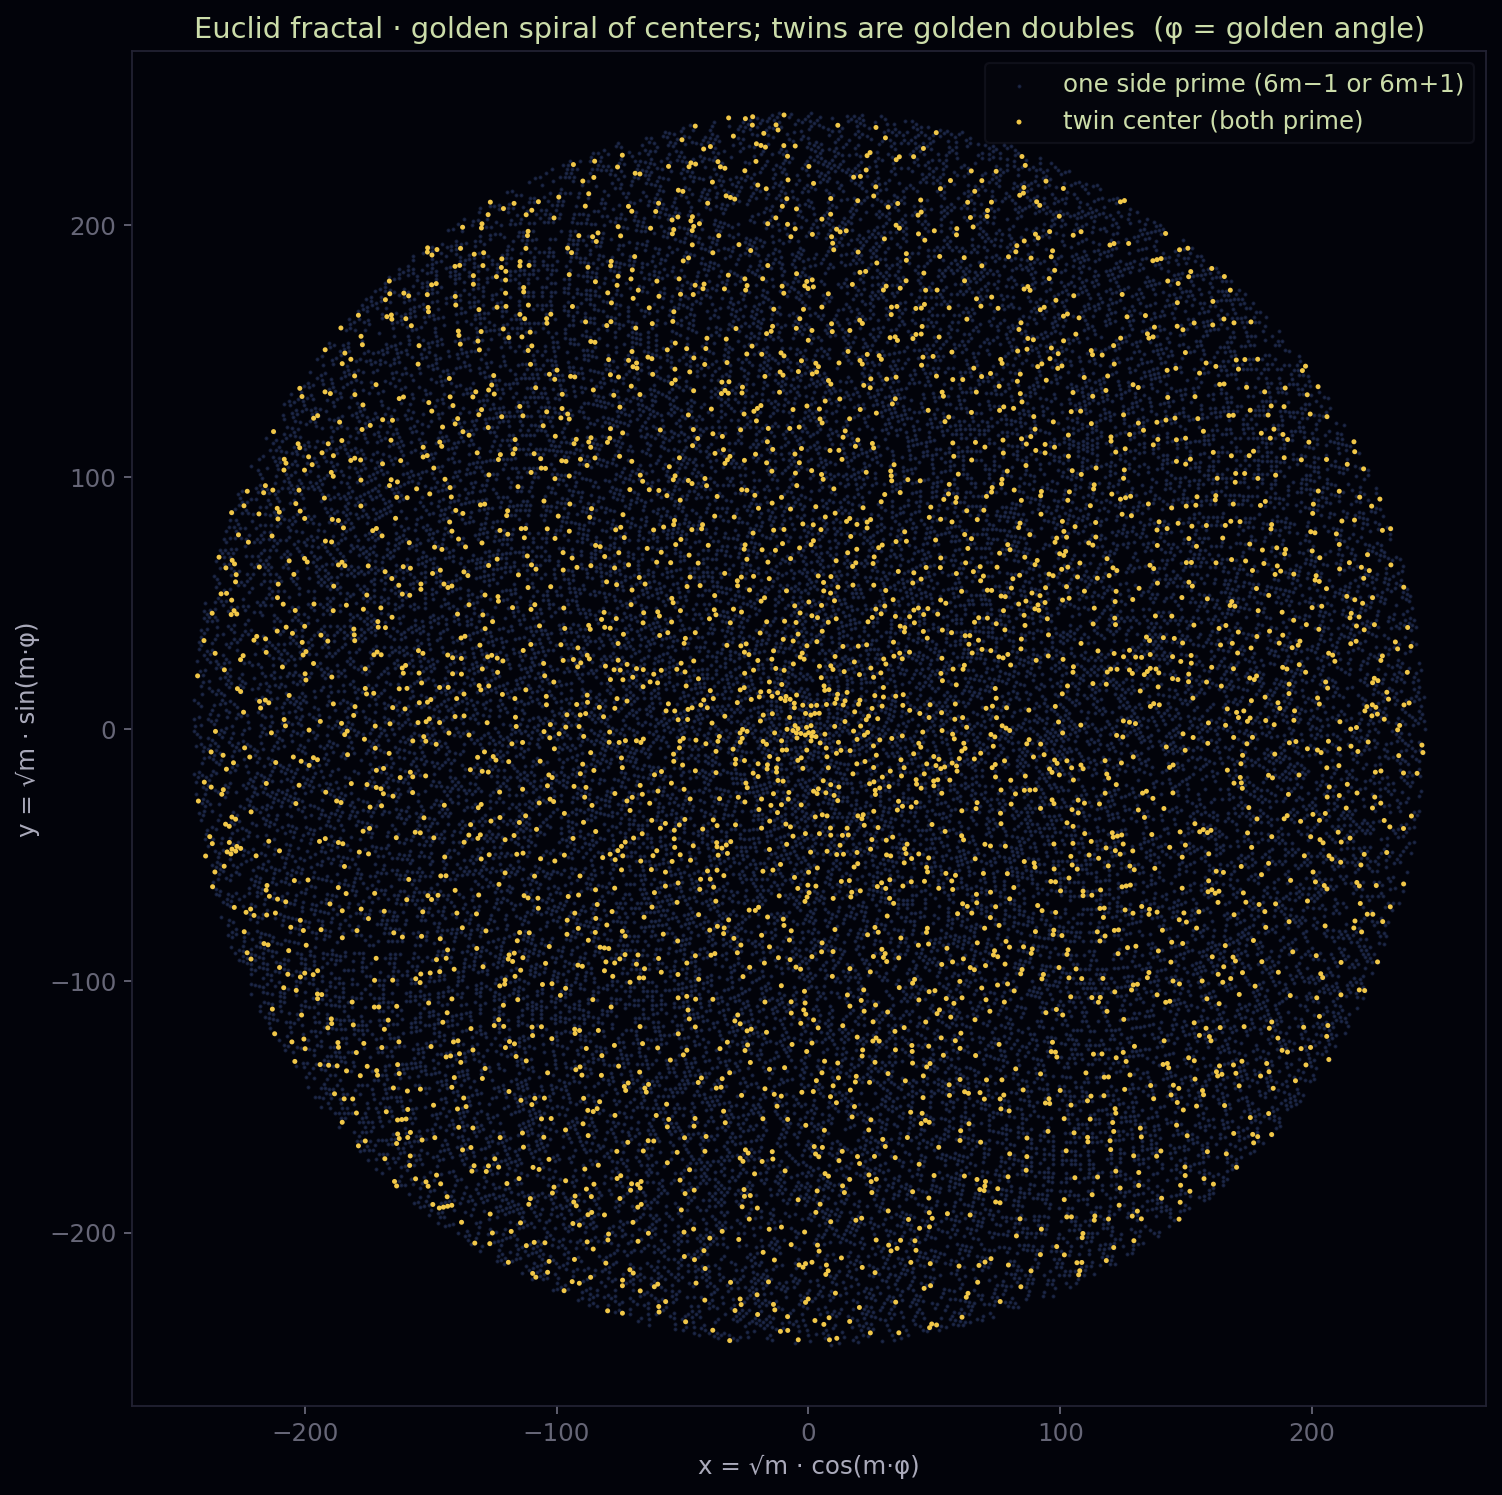
\includegraphics[width=\linewidth]{figures/3_twin_spiral.png}
  \caption{Золотая спираль центров; twin-центры --- золотые двойные точки.}
  \label{fig:twin-spiral}
\end{figure}

\emph{Алгоритм генерации (рис.~\ref{fig:twin-spiral}).} Источник:
\srcpath{tools/fractal/euclid\_fractal.py::twin\_spiral}. Для каждого центра
$m=1,\dots,M-1$ (по умолчанию $M=60000$) точка ставится по золотой спирали
\begin{equation}\label{eq:golden-spiral}
  x=\sqrt{m}\,\cos(m\varphi),\qquad
  y=\sqrt{m}\,\sin(m\varphi),\qquad
  \varphi=\pi(3-\sqrt5),
\end{equation}
где $\varphi$ --- золотой угол. Центр помечается как одна из сторон-простое,
если $6m-1$ или $6m+1$ просто (тускло-синие точки), и как twin-центр, если
просты обе стороны $6m\pm1$ (крупные золотые точки). Радиус $\sqrt m$ даёт
равномерную плотность по площади; цвет постоянен для каждого класса.

\begin{figure}[htbp]
  \centering
  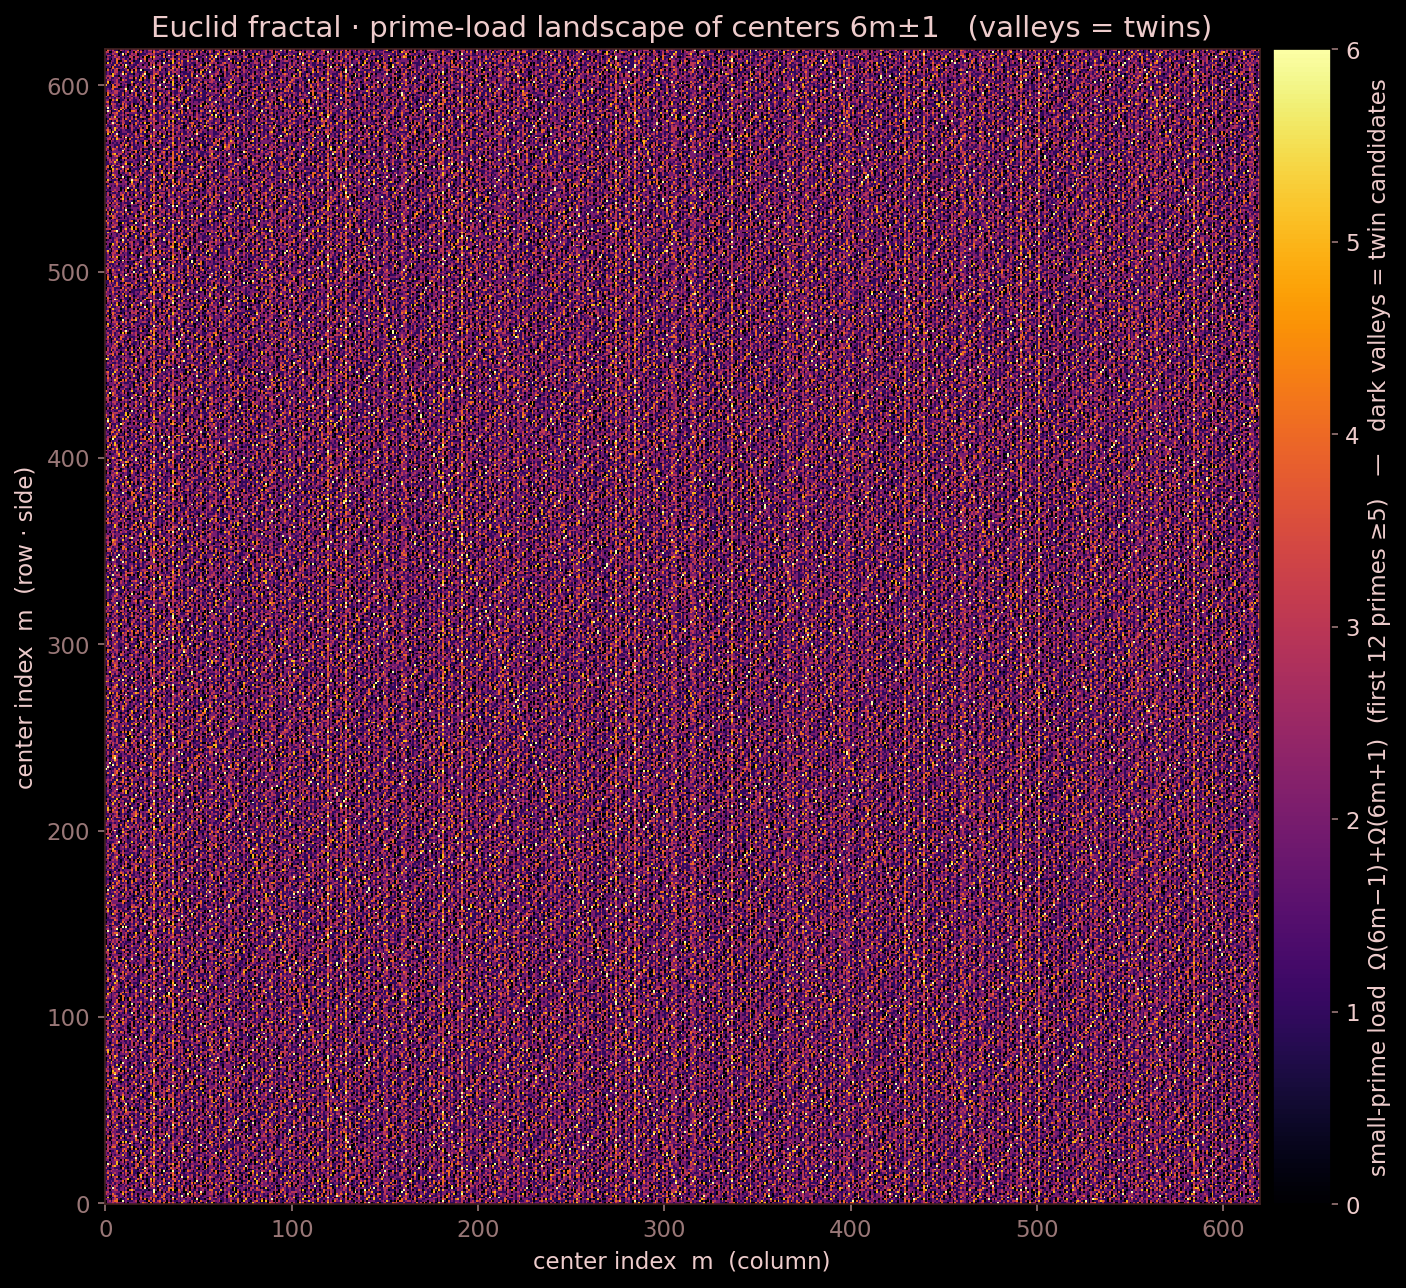
\includegraphics[width=\linewidth]{figures/4_descent_landscape.png}
  \caption{Ландшафт простой нагрузки центров $6m\pm1$; тёмные долины ---
  кандидаты в близнецы.}
  \label{fig:descent-landscape}
\end{figure}

\emph{Алгоритм генерации (рис.~\ref{fig:descent-landscape}).} Источник:
\srcpath{tools/fractal/euclid\_fractal.py::descent\_landscape}. Для каждого центра
$m=0,1,\dots,S^2-1$, разложенного на растр $S\times S$ ($S=620$, построчно по
$m$), вычисляется малопростая нагрузка
\begin{equation}\label{eq:small-prime-load}
  L(m)\;=\;\Omega_B(6m-1)+\Omega_B(6m+1),
\end{equation}
где $\Omega_B(x)$ --- число простых делителей $x$, считаемых с кратностью и
ограниченных первыми $B=12$ простыми $\ge5$ (то есть $5,7,11,\dots,41$). Цвет
ячейки задаётся значением $L(m)$ (палитра inferno, отсечка по 99-му
перцентилю). Центры-близнецы --- где обе стороны $6m\pm1$ просты --- имеют
$L(m)=0$ и образуют тёмные долины; самоподобный рельеф есть
китайско-остаточная периодичность малых простых.

\begin{figure}[htbp]
  \centering
  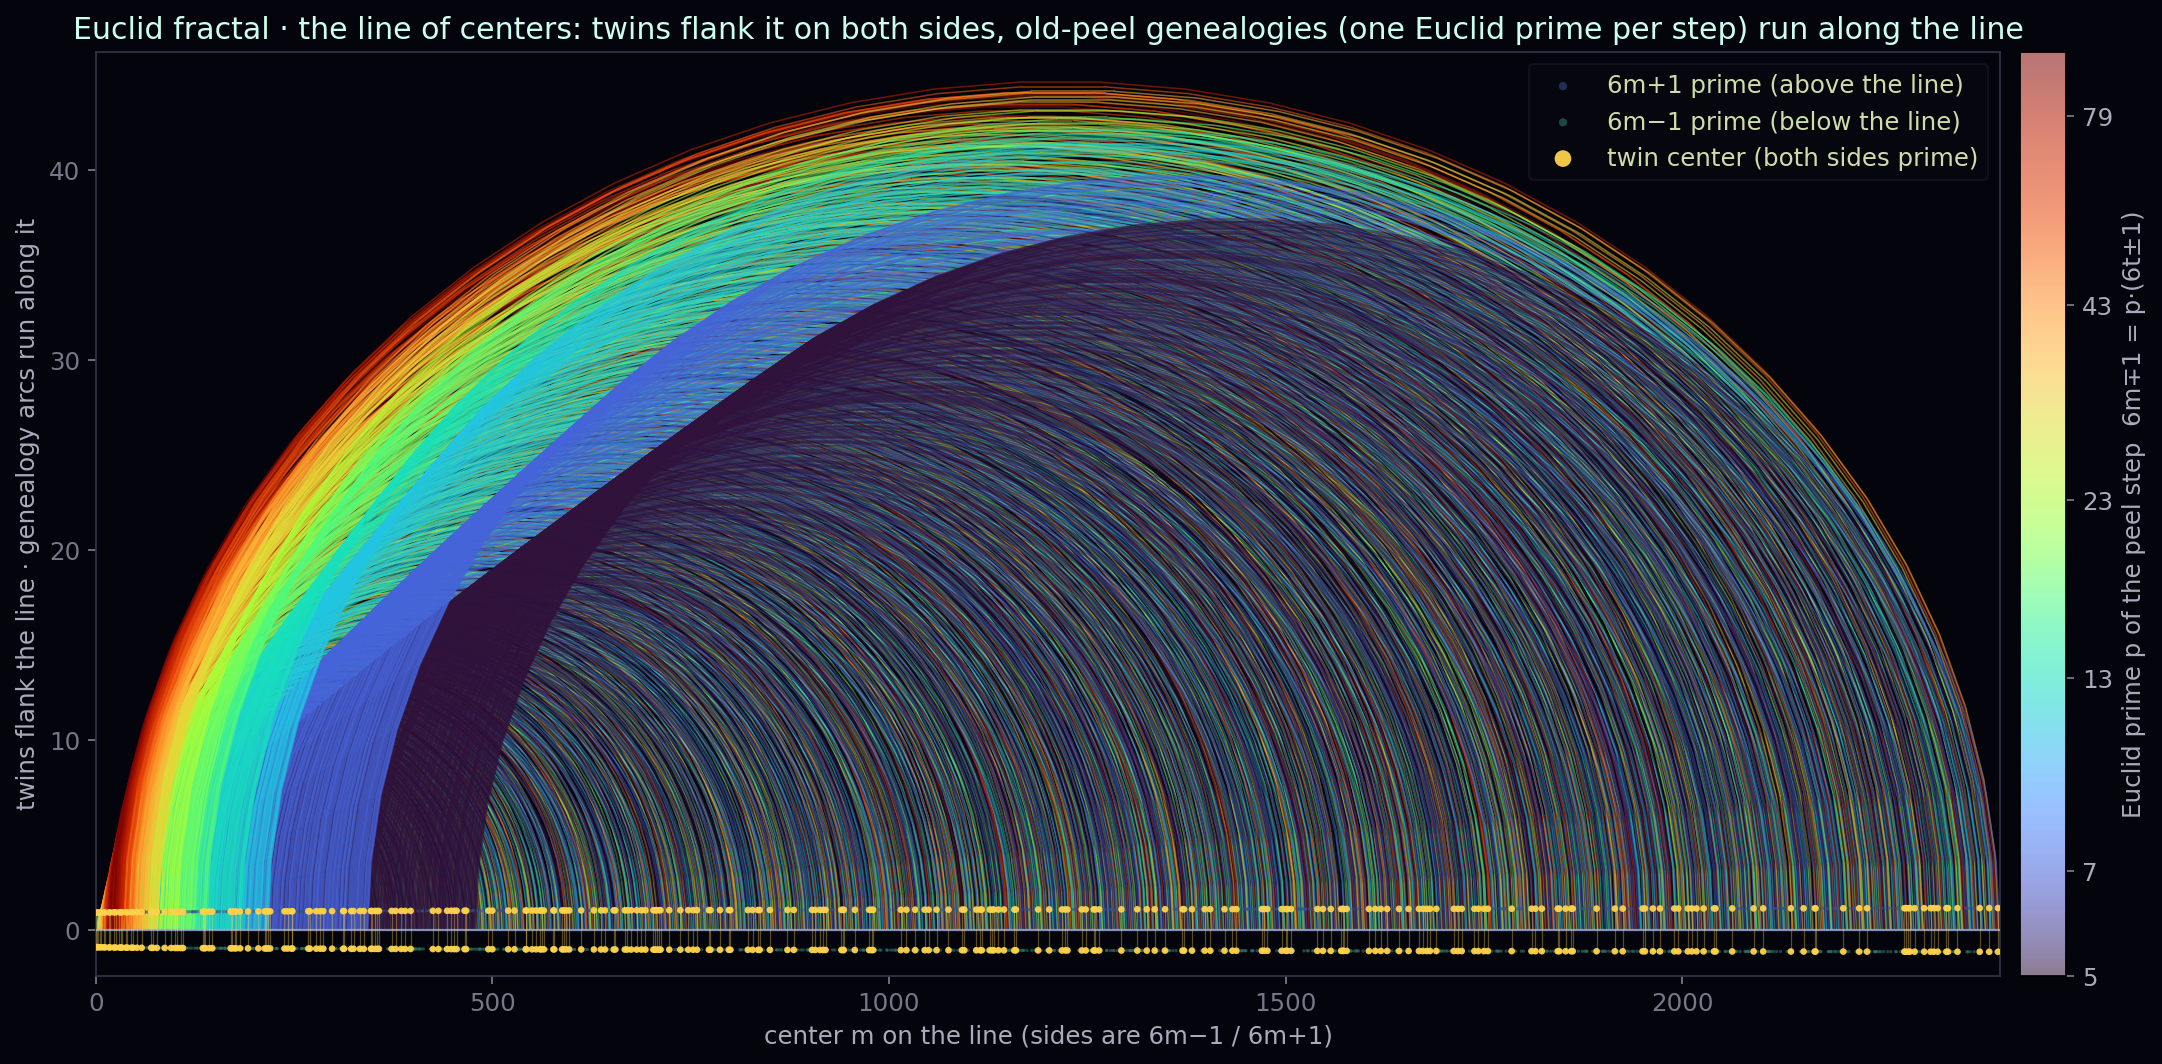
\includegraphics[width=\linewidth]{figures/5_twin_line_genealogy.png}
  \caption{Линия центров: близнецы обрамляют её с двух сторон, old-peel-
  генеалогии (одно евклидово простое на шаг) идут вдоль неё.}
  \label{fig:twin-line-genealogy}
\end{figure}

\emph{Алгоритм генерации (рис.~\ref{fig:twin-line-genealogy}).} Источник:
\srcpath{tools/fractal/euclid\_fractal.py::twin\_line\_genealogy}. Центры
$m=1,\dots,M$ ($M=2400$) откладываются вдоль горизонтальной оси $y=0$. Сторона
$6m+1$ отмечается точкой \emph{над} линией на высоте
$\mathrm{wing}(m)=0.9+0.25\sqrt{m/M}$, сторона $6m-1$ --- симметричной точкой
под линией, когда соответствующее число просто (решето до $6M+2$). Twin-центр
(обе стороны просты) отмечается золотой вертикалью
$[-\mathrm{wing},\,+\mathrm{wing}]$ с точками на концах. Вдоль линии для каждого
$m$ вычисляется old-peel-шаг: если $6m\mp1=p\,(6t\pm1)$ с простым свидетелем
Евклида $p\in[5,97]$, рисуется полуокружностная дуга $m\to t$ высотой
$h=0.06\,|m-t|^{0.85}+0.4$ (36 точек,
$x=\tfrac{m+t}{2}+\tfrac{|m-t|}{2}\cos\theta$, $y=h\sin\theta$,
$\theta\in[0,\pi]$), окрашенная по $\log p$ (палитра turbo). Twin-центры живут
\emph{вне} линии, генеалогия --- \emph{на} ней.

\begin{figure}[htbp]
  \centering
  \includegraphics[width=\linewidth]{figures/6_genealogy_ornament.png}
  \caption{Генеалогический орнамент: полный old-peel-спуск каждого центра,
  сплетённый хордами на окружности центров.}
  \label{fig:genealogy-ornament}
\end{figure}

\emph{Алгоритм генерации (рис.~\ref{fig:genealogy-ornament}).} Источник:
\srcpath{tools/fractal/euclid\_fractal.py::genealogy\_ornament} ($M=4200$,
$\mathrm{PMAX}=97$, $\mathrm{DEPTH}=10$). Центры $1,\dots,M$ сидят на единичной
окружности под углом $2\pi m/M$. Для каждого центра полная old-peel-генеалогия
$m\to t_1\to t_2\to\cdots$ (до глубины $10$) строится шагом
$6k\mp1=p\,(6t\pm1)$: каждый шаг --- хорда Безье с контрольной точкой
$\tfrac12(P_a+P_b)\cdot(1-0.92\min(2\Delta\theta,1))$, где
$\Delta\theta=|a-b|/M$ (длинные хорды ныряют глубже к центру); цвет по
$\log p$ (turbo). Twin-центры (пустая генеалогия) сидят на ободе золотыми
точками.

Два оставшихся рисунка --- концептуальные: они помещают \emph{реальную}
генеалогию в космологическую картину. Подчеркнём честную границу в точности,
как в коде: строго доказаны здесь лишь необратимость времени и кривизна
пространства (невозможность двигателя из \cref{sec:engine}); прочтение
картинок как физики --- перевод, а не теорема.

\begin{figure}[htbp]
  \centering
  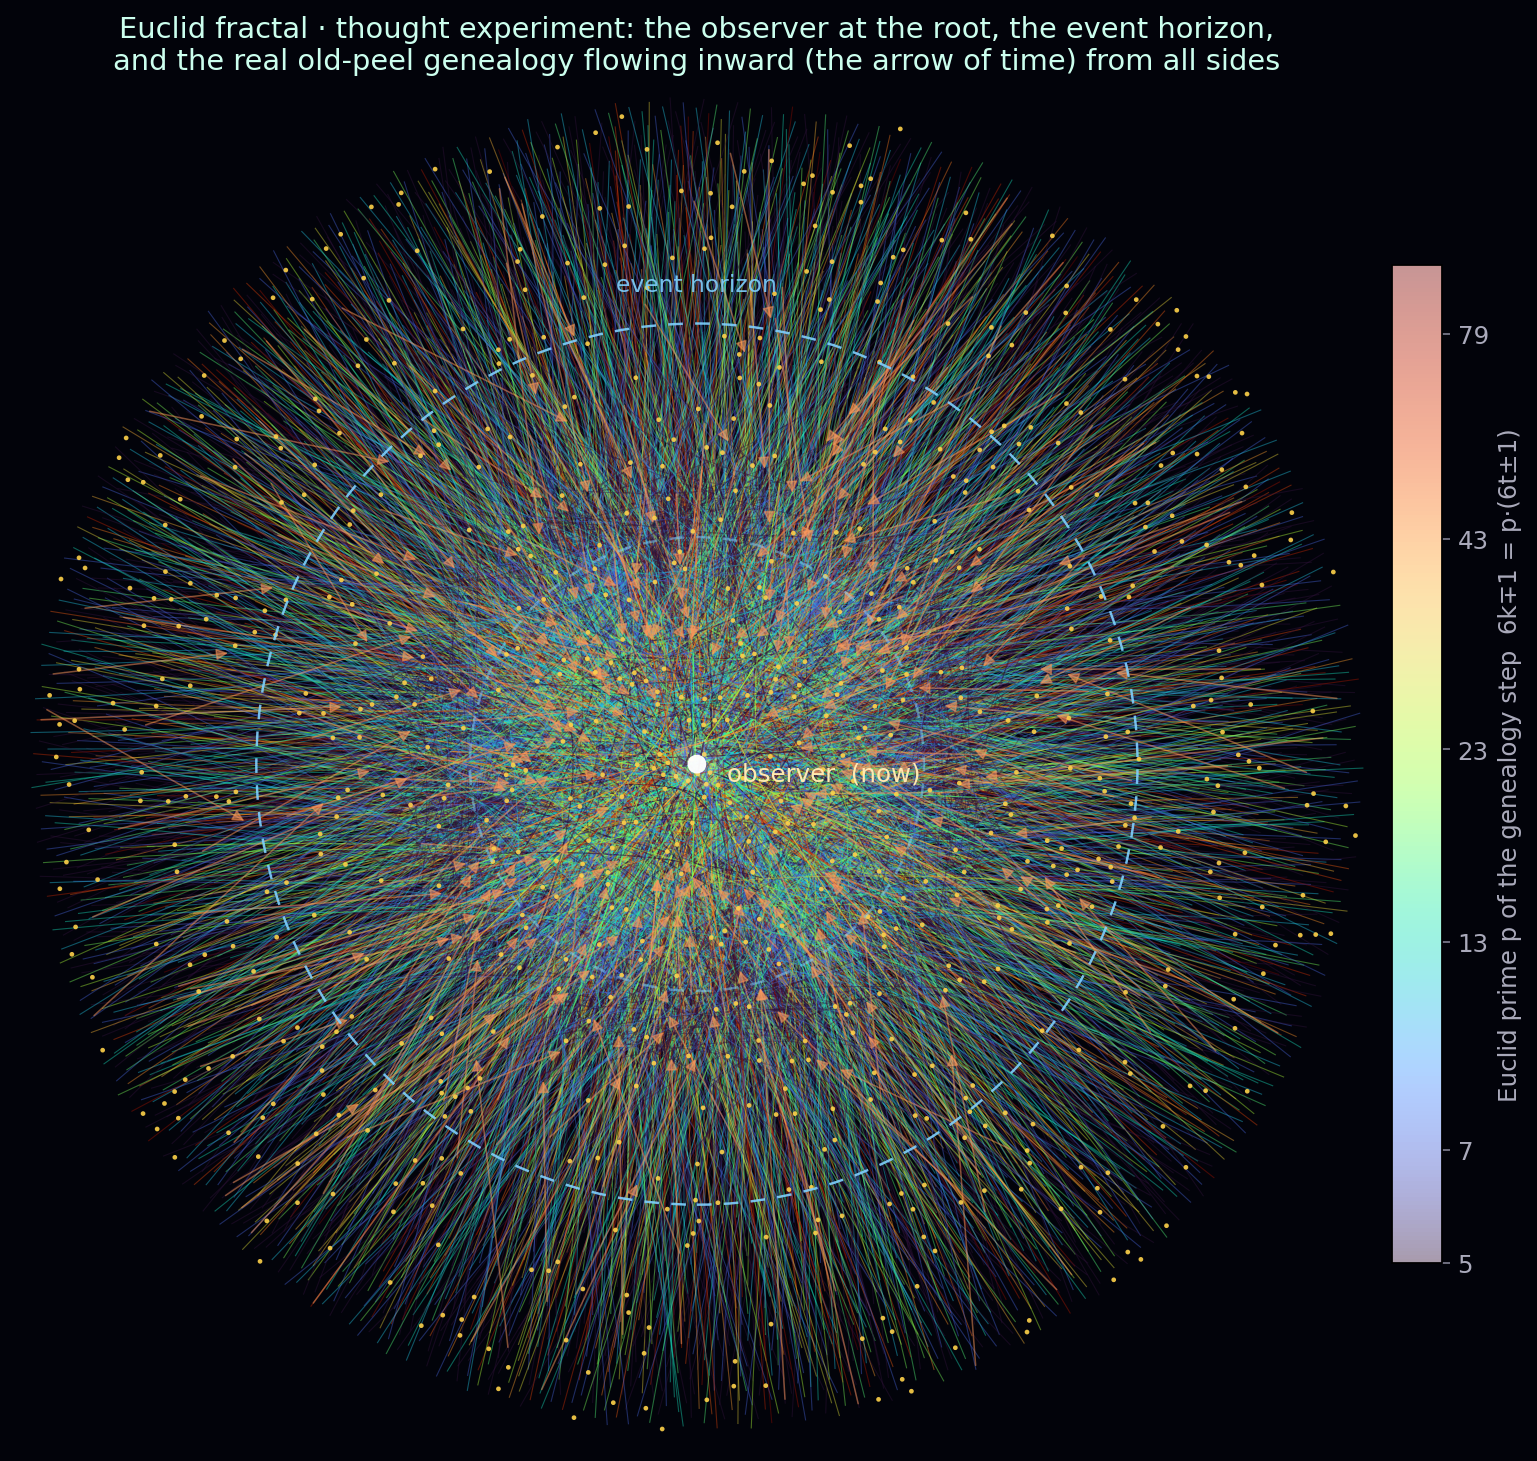
\includegraphics[width=\linewidth]{figures/7_observer_horizon.png}
  \caption{Мысленный эксперимент: наблюдатель у корня, горизонт событий и
  реальная old-peel-генеалогия, текущая внутрь (стрела времени).}
  \label{fig:observer-horizon}
\end{figure}

\emph{Алгоритм генерации (рис.~\ref{fig:observer-horizon}).} Источник:
\srcpath{tools/fractal/euclid\_cosmology.py::observer\_horizon} ($M=9000$,
$\mathrm{PMAX}=97$, $\mathrm{DEPTH}=9$). Центр $k$ размещается на золотой спирали
по радиусу-высоте $r=\sqrt{k/M}$, угол $k\varphi$ ($\varphi$ --- золотой угол):
малые $k$ у центра (наблюдатель), большие --- на периферии. Полная
old-peel-генеалогия каждого центра строится шагом $6k\mp1=p\,(6t\pm1)$
(наименьшее простое-делитель $p\in[5,97]$ композитной стороны, $t<k$),
итерируемым до глубины $9$. Каждый шаг $k\to t$ рисуется квадратичной кривой
Безье с контрольной точкой $\tfrac12(P_k+P_t)\cdot0.72$, подтянутой к началу
(дуга ныряет внутрь); цвет по $\log p$ (палитра turbo). Оранжевые стрелки
ставятся на реальных первых шагах с $r>0.30$ и указывают от $k$ к $t$ (внутрь).
Пунктирные окружности радиусов $0.66$ и $0.34$ --- горизонт событий; золотые
точки --- twin-центры.

\begin{figure}[htbp]
  \centering
  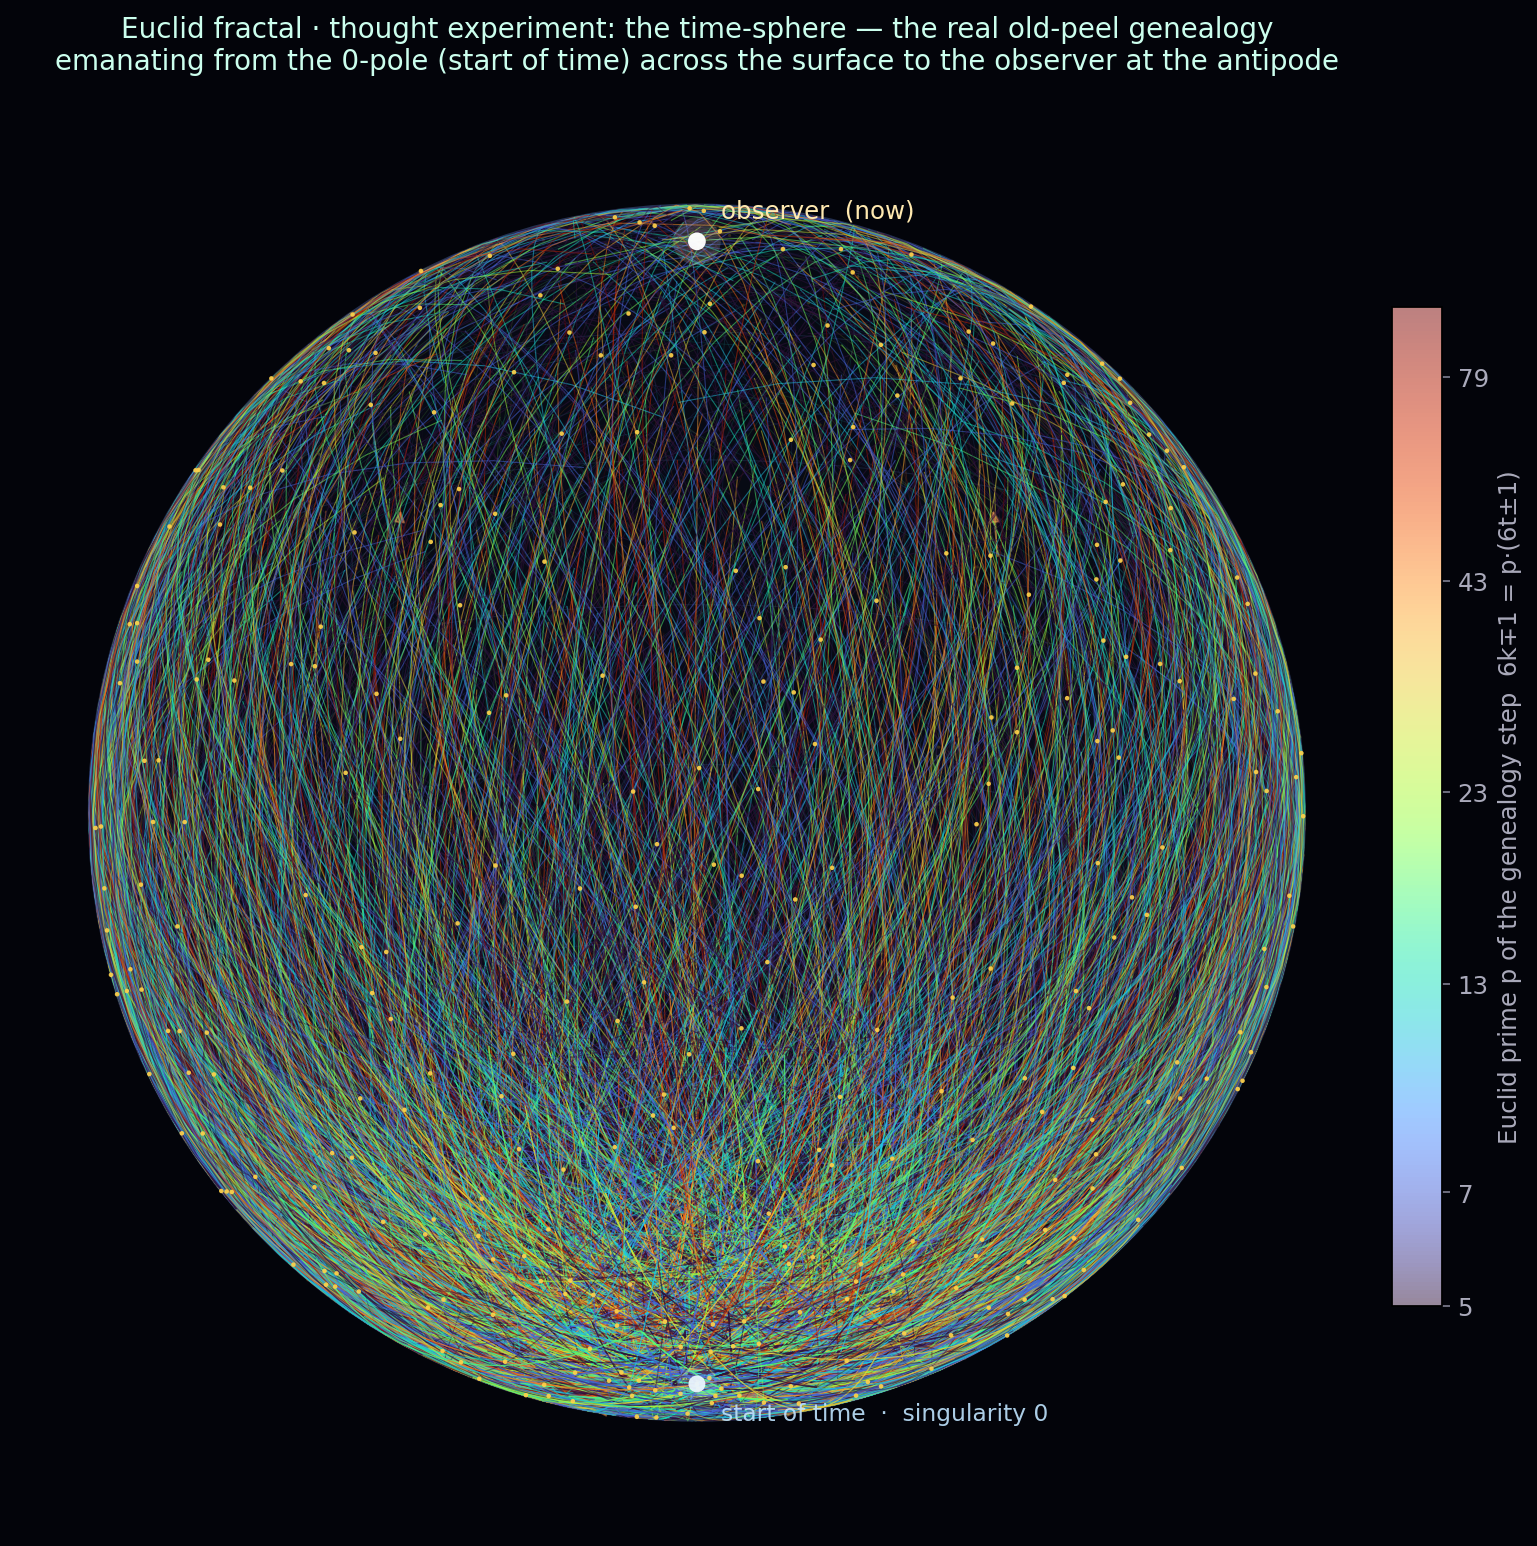
\includegraphics[width=\linewidth]{figures/8_time_sphere.png}
  \caption{Мысленный эксперимент: сфера времени --- реальная
  old-peel-генеалогия, исходящая из полюса-$0$ (старт времени) к наблюдателю в
  антиподе.}
  \label{fig:time-sphere}
\end{figure}

\emph{Алгоритм генерации (рис.~\ref{fig:time-sphere}).} Источник:
\srcpath{tools/fractal/euclid\_cosmology.py::time\_sphere} ($M=7000$,
$\mathrm{PMAX}=97$, $\mathrm{DEPTH}=9$). Центр $k$ отображается в единичный
вектор на сфере: высота $z=-1+2(k-1)/(M-1)$ (так $k=1$ --- в полюсе-$0$,
$z=-1$; $k=M$ --- в полюсе-наблюдателе, $z=+1$), долгота $k\varphi$ по золотому
углу, $\rho=\sqrt{1-z^2}$. Полная old-peel-генеалогия $6k\mp1=p\,(6t\pm1)$
(глубина $9$) рисуется дугами больших кругов (сферический slerp между $V_k$ и
$V_t$); дуги передней полусферы яркие, задней --- тусклые; цвет по $\log p$
(turbo). Проекция --- поворот вокруг оси $x$ на $20^\circ$. Оранжевые стрелки
на меридианах указывают генеративное направление времени от полюса-$0$ к
полюсу-наблюдателю; золотые точки --- twin-центры; два полюса подписаны как
«наблюдатель (сейчас)» и «старт времени $\cdot$ сингулярность $0$».
